\documentclass{article}

\title{CSCI 3461: Databases\\Term Project}

\author{Evan Farrell, Jordan Dempsey \& Tyler Robinson}

\usepackage[textwidth=\textwidth,textheight=\textheight,margin=1in]{geometry}
\usepackage{listingsutf8}
\usepackage{graphicx   }
\usepackage{titlesec  }
\usepackage{amssymb }
\usepackage{amsmath}
\usepackage{float}
% \usepackage{pifont}
\usepackage{color}
\usepackage{subcaption}
\usepackage{url}
\usepackage{ulem}
\usepackage{accsupp}
\usepackage{chngcntr}
\usepackage[hidelinks]{hyperref}
\hypersetup{
    colorlinks=true, %set true if you want colored links
    linktoc=all,     %set to all if you want both sections and subsections linked
    linkcolor=blue,  %choose some color if you want links to stand out
    urlcolor=blue,
}
\renewcommand{\thesubsection}{\thesection.\alph{subsection}}
% \newcommand{\noaccsupp}[1]{\BeginAccSupp{ActualText={}}#1\EndAccSupp{}}

% \titleformat{\section}[runin]
%   {\normalfont\Large\bfseries}{\thesection}{1em}{}
% \titleformat{\subsection}[runin]
%   {\normalfont\large\bfseries}{\thesubsection}{1em}{}

\newcommand{\cmark}{\ding{51}}%
\newcommand{\xmark}{\ding{55}}%
\newcommand{\arrow}{\ding{217}}%

\lstdefinestyle{scilab}
{
    language={scilab},
    basicstyle=\footnotesize\tt,
    commentstyle=\color[rgb]{0.5,0.5,0.5},
    stringstyle=\color[rgb]{0.13,0.54,0.13},
    backgroundcolor=\color[rgb]{0.95,0.94,0.87},
    keywordstyle=\color{blue},
    keywordstyle=[2]\color[rgb]{0.0, 0.7, 0.7}\textit,
    keywordstyle=[3]\color[rgb]{0.1, 0.4, 0.9}\emph,
    otherkeywords={barycentric,interpolation\_sin,interpolation\_runge,interpolation\_bary\_runge,interpolation\_error,cheby,question\_2\_a,question\_2\_b,question\_3\_a,question\_3\_b,question\_3\_c,question\_4\_a,question\_4\_b,question\_4\_c,runge,lagrange,intrpl_err_wi,question_2_b_2},
    morekeywords=[2]{question\_2\_a,question\_2\_b,question\_3\_a,question\_3\_b,question\_3\_c,question\_4\_a,question\_4\_b,question\_4\_c,question\_2\_b\_2},
    morekeywords=[3]{lagrange,barycentric,interpolation\_sin,interpolation\_runge,interpolation\_bary\_runge,runge,interpolation\_error,cheby,intrpl_err_wi},
    numbers=left,
    stepnumber=1,
    frame=single
}
\newcommand{\noncopynumber}[1]{%
    \BeginAccSupp{method=escape,ActualText={}}%
    #1%
    \EndAccSupp{}%
}

\lstnewenvironment{scilab}
{\lstset{
style=scilab,
numberstyle=\tiny\color[rgb]{.5,.5,.5}\noncopynumber,
}}
{}

\lstnewenvironment{scilab_compact}
{\lstset{
style=scilab,
numbers=none,
basicstyle=\tiny
}}
{}

\counterwithin{figure}{section}
\graphicspath{ {figures/} }

\begin{document}

\maketitle
\clearpage
\section{Database Diagrams}
\begin{figure}[H]
  \center
  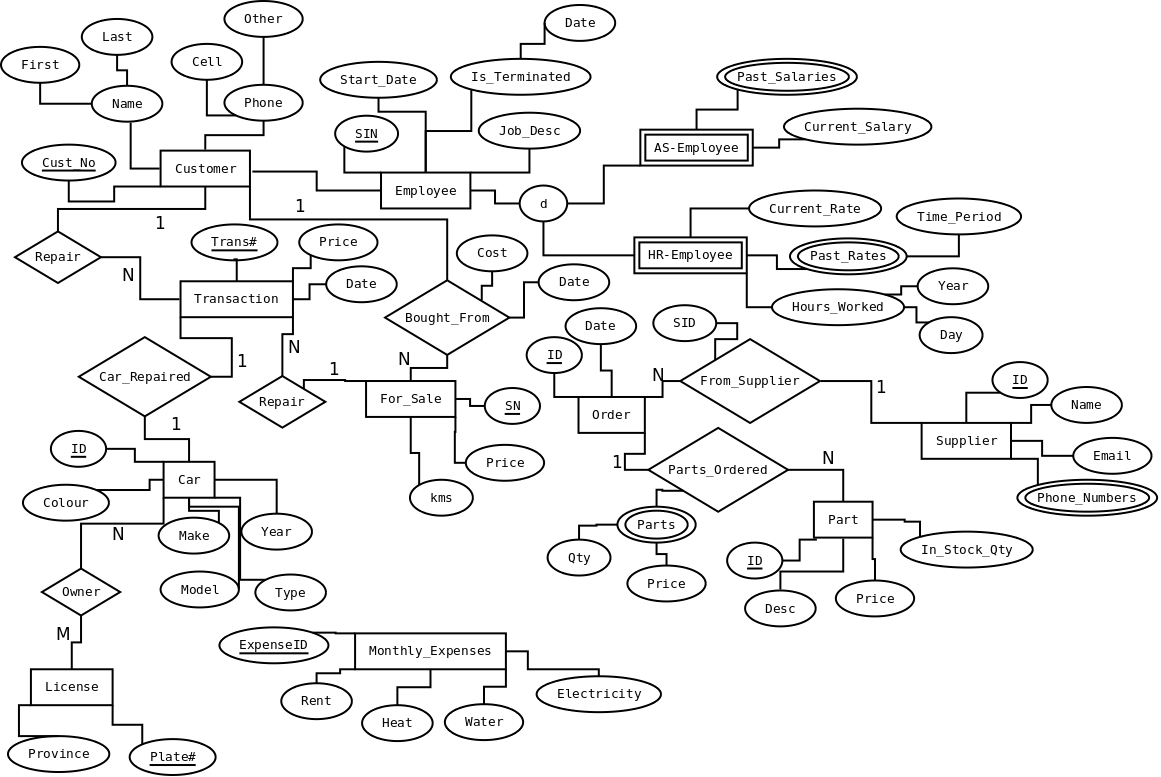
\includegraphics[width=.9\linewidth]{eer.png}
  \caption{MUC EER Diagram.}
  \label{fig:eer}
\end{figure}
\bigskip

\begin{figure}[H]
  \center
  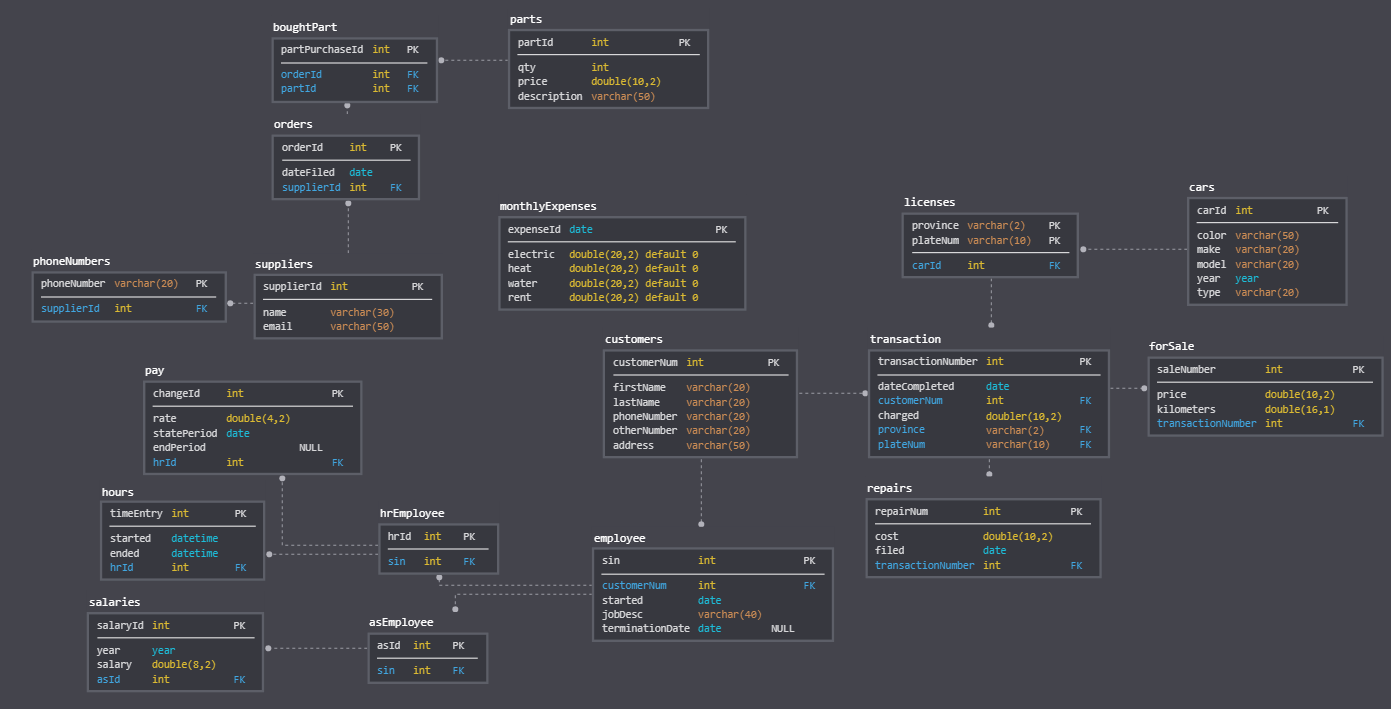
\includegraphics[width=.9\linewidth]{rds.png}
  \caption{MUC Relational Database Schema.}
  \label{fig:rds}
\end{figure}

\clearpage
\section{Description}
To keep track of it's many (happy) customers, MUC employs a large number of technologies into it's \href{http://csci3461.cs.smu.ca/~tj_robinson/}{website}. The web-app is written predominately in Javascript code (ECMAscript 2015) with additional PHP and CSS variants to aid in visuals and clarity. \\

The client-side is responsible for generating queries to the MySQL database serverside. While this is potentially the least secure way possible to perform this task, it was also the fastest for prototyping and researching. \\

The site is organized into a few folders\footnote{\texttt{/external} contains the files to rebuild and autopopulate the database from scratch.}:\\

\begin{tabular}{|l|l|}
\hline
\texttt{common} & HTML shared among many pages, including the \texttt{head} section. \\
\texttt{css} & Exclusively CSS, completely generated.\\
\texttt{external} & Tools \& scripts for use on the server with no access from the web. \\
\texttt{images} & Visual data for the website.\\
\texttt{sass} & SASS source files to be interpreted into raw CSS. \\
\texttt{report} & Source for this document. \\
\texttt{scripts} & PHP and JS functions  to support the web-app.\\
\hline
\end{tabular}
\\

Outside of these subdirectories, the files located in the home directory are all loadable webpages, the first of which being \texttt{index.php}. It's important to note that despite the PHP extension, the extent of the languages use in this case is limited to includes.\\

\begin{tabular}{|l|l|}
\hline
\texttt{index.php} & First page and location to view full tables. \\
\texttt{edit.php} & Manual management of the various tables.\\
\texttt{cancel.php} & Cancelling previous orders. \\
\texttt{order.php} & Creating and submitting new parts orders.\\
\texttt{supplier.php} & Adding new suppliers into the database. \\
\hline
\end{tabular}
\vspace{.5cm}

Inside the scripts folder, the key files to look at would be:
\begin{itemize}
    \item \texttt{db.php}: Routing MySQL calls to the database and returning JSON replies.
    \item \texttt{db.js}: Includes \texttt{sendRequest(...)}, which communicates asynchronously with \texttt{db.php} to avoid random page loads between requests.
    \item \texttt{helpers.js}: Includes a few common functions, including creating a table based on a database response for a query.
\end{itemize}
The remainder of the files are related directly to the page they appear on; there is no overlap between the remaining scripts.\\

Additional technologies/libraries used in the creation of the web-app include \texttt{jQuery}, \texttt{bootstrap} (with CSS), \texttt{popper.js} and \texttt{velocity.js}.
\end{document}
